\documentclass{standalone}
\usepackage{tikz}
\usepackage{ctex,siunitx,upgreek}
\setCJKmainfont{Noto Serif CJK SC}
\usepackage{tkz-euclide}
\usepackage{amsmath,amsfonts,amssymb}
\usetikzlibrary{patterns, calc,3d}
\usetikzlibrary {decorations.pathmorphing,decorations.pathreplacing,decorations.shapes}
\tikzset{label style/.append style={font=\small}}
\begin{document}
\small
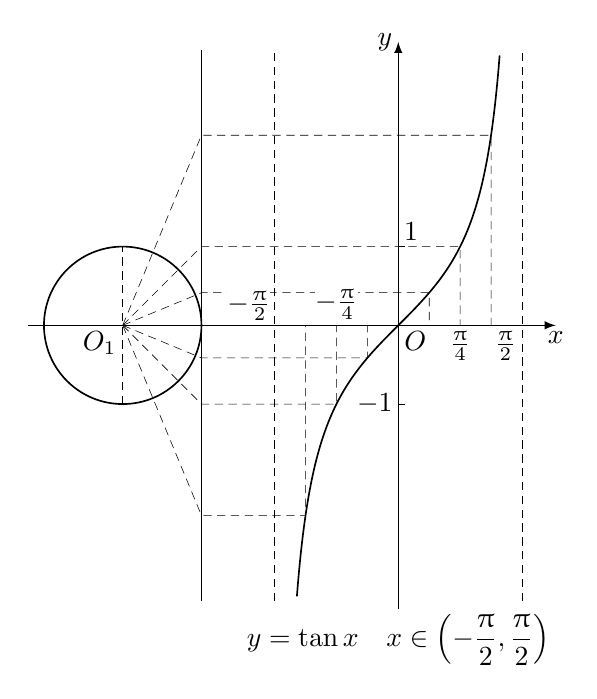
\begin{tikzpicture}[>=latex,scale=1.0,inner sep=2pt]
  \draw[->](-4.7,0)--(2.0,0)node[below]{$x$};
  \draw[->](0,-3.6)node[below]{$y=\tan x\quad x\in\left(-\dfrac\uppi2,\dfrac\uppi2\right)$}--(0,3.6)node[left]{$y$};
  \node at (0,0)[below right]{$O$};
  \draw[semithick](-3.5,0)node[below left]{$O_1$}circle(1);
  \draw(-2.5,-3.5)--++(0,7);
  \draw[very thin,densely dashed](-3.5,-1)--(-3.5,1);
  \draw[semithick,samples=200,domain=-0.41*pi:0.41*pi]plot(\x,{tan(\x r)});
  \foreach \x/\y in {-1/left,1/above right}
  {
    \draw[very thin,densely dashed](\x*pi/2,-3.5)--++(0,7);
    \draw[very thin](0,\x)node[\y]{$\x$}--++(0.08,0);
  }
  \foreach \x in {1,2,3} 
  {
    \draw[very thin,densely dashed](-3.5,0)--(-2.5,{tan(\x*22.5)})--({\x*pi/8},{tan(\x*22.5)})--({\x*pi/8},0);
    \draw[very thin,densely dashed](-3.5,0)--(-2.5,{-tan(\x*22.5)})--({-\x*pi/8},{-tan(\x*22.5)})--({-\x*pi/8},0);
  }
  \node at (pi/2,0)[below left]{$\frac\uppi2$};
  \node at (-pi/2,0)[above left=2pt,inner sep=0pt,fill=white]{$-\frac\uppi2$};
  \node at (0.25*pi,0)[below]{$\frac{\uppi}4$};
  \node at (-0.25*pi,0)[above=2pt,inner sep=0pt,fill=white]{$-\frac{\uppi}4$};
\end{tikzpicture}
\end{document}